\begin{figure}[h!]
\centering
% Thesis-wide categorical color palette
% Usage: % Thesis-wide categorical color palette
% Usage: % Thesis-wide categorical color palette
% Usage: \input{figures/palette} in any figure file
%
% Muted primary colors -- print-friendly, visually distinct.
% Inspired by Cooper Union's red/blue primaries, softened for
% academic figures. Use palA-palC for data series in scatter
% plots, line charts, bar charts, etc.

\definecolor{palA}{HTML}{1F77B4}   % Tableau blue
\definecolor{palB}{HTML}{D62728}   % Tableau red
\definecolor{palC}{HTML}{2CA02C}   % Tableau green
 in any figure file
%
% Muted primary colors -- print-friendly, visually distinct.
% Inspired by Cooper Union's red/blue primaries, softened for
% academic figures. Use palA-palC for data series in scatter
% plots, line charts, bar charts, etc.

\definecolor{palA}{HTML}{1F77B4}   % Tableau blue
\definecolor{palB}{HTML}{D62728}   % Tableau red
\definecolor{palC}{HTML}{2CA02C}   % Tableau green
 in any figure file
%
% Muted primary colors -- print-friendly, visually distinct.
% Inspired by Cooper Union's red/blue primaries, softened for
% academic figures. Use palA-palC for data series in scatter
% plots, line charts, bar charts, etc.

\definecolor{palA}{HTML}{1F77B4}   % Tableau blue
\definecolor{palB}{HTML}{D62728}   % Tableau red
\definecolor{palC}{HTML}{2CA02C}   % Tableau green

\definecolor{agentblue}{HTML}{4C72B0}
\definecolor{rewardgreen}{HTML}{55A868}
\vspace{0.5em}

\tikzset{
    dg cell/.style={minimum size=1.0cm, draw=black!40, thick},
    dg reward/.style={font=\scriptsize\bfseries},
    dg agent/.style={circle, draw=agentblue, thick,
                     fill=agentblue!20, inner sep=2.5pt},
    dg ghost/.style={circle, draw=agentblue, thick,
                     fill=agentblue!12, inner sep=2.5pt},
    dg chev/.style={semithick, agentblue!50},
    dg slbl/.style={font=\tiny, text=black!30, anchor=north west},
    % Tree styles
    dt node/.style={circle, draw=black!40, thick,
                    minimum size=0.7cm, font=\scriptsize},
    dt start/.style={dt node, draw=agentblue, fill=agentblue!15},
    dt taken/.style={-, thick, black!45},
    dt faded/.style={-, thick, black!18, dashed},
    dt ann/.style={font=\small, text=black!60},
    dt fann/.style={font=\small, text=black!28},
    dt note/.style={font=\tiny, text=black!28},
}

%% Panel (a): Low gamma -- short path preferred
\begin{subfigure}{\textwidth}
\centering
\begin{minipage}[c]{0.32\textwidth}
\centering
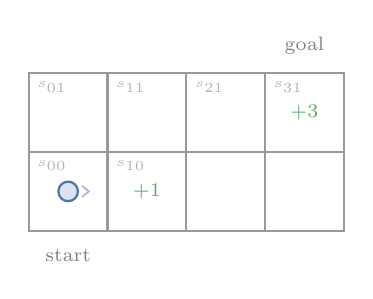
\begin{tikzpicture}
    \def\ds{1.0}
    % Row 0 (bottom)
    \node[dg cell] (g00) at (0, 0) {};
    \node[dg cell] (g10) at (\ds, 0) {};
    \node[dg cell] (g20) at (2*\ds, 0) {};
    \node[dg cell] (g30) at (3*\ds, 0) {};
    % Row 1 (top)
    \node[dg cell] (g01) at (0, \ds) {};
    \node[dg cell] (g11) at (\ds, \ds) {};
    \node[dg cell] (g21) at (2*\ds, \ds) {};
    \node[dg cell] (g31) at (3*\ds, \ds) {};
    % State labels (all path-relevant cells)
    \node[dg slbl] at (g00.north west) {$s_{00}$};
    \node[dg slbl] at (g10.north west) {$s_{10}$};
    \node[dg slbl] at (g01.north west) {$s_{01}$};
    \node[dg slbl] at (g11.north west) {$s_{11}$};
    \node[dg slbl] at (g21.north west) {$s_{21}$};
    \node[dg slbl] at (g31.north west) {$s_{31}$};
    % Rewards
    \node[dg reward, text=rewardgreen] at (g10) {$+1$};
    \node[dg reward, text=rewardgreen] at (g31) {$+3$};
    % Agent at start with right chevron (going to +1)
    \node[dg agent] at (g00) {};
    \draw[dg chev]
          ([xshift=5pt, yshift=2pt]g00.center) --
          ([xshift=7.5pt]g00.center) --
          ([xshift=5pt, yshift=-2pt]g00.center);
    % Start and goal labels
    \node[font=\scriptsize, text=black!50, below=3pt]
        at (g00.south) {start};
    \node[font=\scriptsize, text=black!50, above=3pt]
        at (g31.north) {goal};
\end{tikzpicture}
\end{minipage}%
\hfill
\begin{minipage}[c]{0.62\textwidth}
\centering
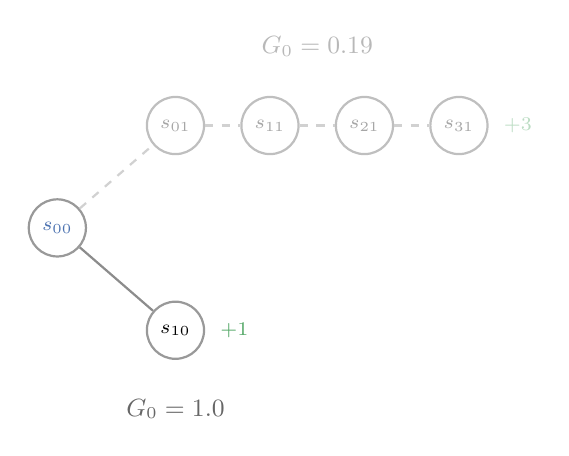
\begin{tikzpicture}
    % Start
    \node[dt node, font=\scriptsize\bfseries, text=agentblue]
        (s0) at (0, 0) {$s_{00}$};
    % Short path (taken)
    \node[dt node] (r1) at (1.5, -1.3) {$s_{10}$};
    \node[dg reward, text=rewardgreen, right=2pt] at (r1.east)
        {$+1$};
    \draw[dt taken] (s0) -- (r1);
    % Long path (faded)
    \node[dt node, draw=black!25, text=black!35] (t1) at (1.5, 1.3) {$s_{01}$};
    \node[dt node, draw=black!25, text=black!35] (t2) at (2.7, 1.3) {$s_{11}$};
    \node[dt node, draw=black!25, text=black!35] (t3) at (3.9, 1.3) {$s_{21}$};
    \node[dt node, draw=black!25, text=black!35] (r3) at (5.1, 1.3) {$s_{31}$};
    \node[dg reward, text=rewardgreen!40, right=2pt] at (r3.east)
        {$+3$};
    \draw[dt faded] (s0) -- (t1);
    \draw[dt faded] (t1) -- (t2);
    \draw[dt faded] (t2) -- (t3);
    \draw[dt faded] (t3) -- (r3);
    % Return annotations
    \node[dt ann, ] at (1.5, -2.3) {$G_0 = 1.0$};
    \node[dt fann] at (3.3, 2.3) {$G_0 = 0.19$};
\end{tikzpicture}
\end{minipage}
\vspace{0.3em}
\subcaption{$\gamma = 0.5$: the nearby $+1$ is preferred.}
\label{fig:discount-low}
\end{subfigure}

\vspace{0.6em}

%% Panel (b): High gamma -- long path preferred
\begin{subfigure}{\textwidth}
\centering
\begin{minipage}[c]{0.32\textwidth}
\centering
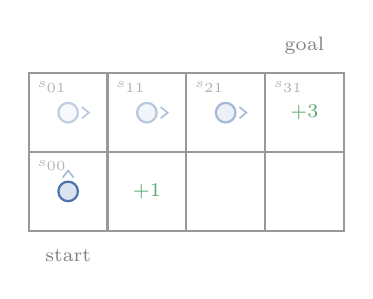
\begin{tikzpicture}
    \def\ds{1.0}
    % Row 0 (bottom)
    \node[dg cell] (g00) at (0, 0) {};
    \node[dg cell] (g10) at (\ds, 0) {};
    \node[dg cell] (g20) at (2*\ds, 0) {};
    \node[dg cell] (g30) at (3*\ds, 0) {};
    % Row 1 (top)
    \node[dg cell] (g01) at (0, \ds) {};
    \node[dg cell] (g11) at (\ds, \ds) {};
    \node[dg cell] (g21) at (2*\ds, \ds) {};
    \node[dg cell] (g31) at (3*\ds, \ds) {};
    % State labels
    \node[dg slbl] at (g00.north west) {$s_{00}$};
    \node[dg slbl] at (g01.north west) {$s_{01}$};
    \node[dg slbl] at (g11.north west) {$s_{11}$};
    \node[dg slbl] at (g21.north west) {$s_{21}$};
    \node[dg slbl] at (g31.north west) {$s_{31}$};
    % Rewards
    \node[dg reward, text=rewardgreen] at (g10) {$+1$};
    \node[dg reward, text=rewardgreen] at (g31) {$+3$};
    % Agent at start with up chevron (taking long path)
    \node[dg agent] at (g00) {};
    \draw[dg chev]
          ([yshift=5pt, xshift=-2pt]g00.center) --
          ([yshift=7.5pt]g00.center) --
          ([yshift=5pt, xshift=2pt]g00.center);
    % Ghost trail
    \node[dg ghost, draw=agentblue!35, fill=agentblue!5]
        at (g01) {};
    \node[dg ghost, draw=agentblue!40, fill=agentblue!7]
        at (g11) {};
    \node[dg ghost, draw=agentblue!50, fill=agentblue!10]
        at (g21) {};
    % Chevrons
    \draw[dg chev, agentblue!40]
          ([xshift=5pt, yshift=2pt]g01.center) --
          ([xshift=7.5pt]g01.center) --
          ([xshift=5pt, yshift=-2pt]g01.center);
    \draw[dg chev, agentblue!45]
          ([xshift=5pt, yshift=2pt]g11.center) --
          ([xshift=7.5pt]g11.center) --
          ([xshift=5pt, yshift=-2pt]g11.center);
    \draw[dg chev, agentblue!50]
          ([xshift=5pt, yshift=2pt]g21.center) --
          ([xshift=7.5pt]g21.center) --
          ([xshift=5pt, yshift=-2pt]g21.center);
    % Start and goal labels
    \node[font=\scriptsize, text=black!50, below=3pt]
        at (g00.south) {start};
    \node[font=\scriptsize, text=black!50, above=3pt]
        at (g31.north) {goal};
\end{tikzpicture}
\end{minipage}%
\hfill
\begin{minipage}[c]{0.62\textwidth}
\centering
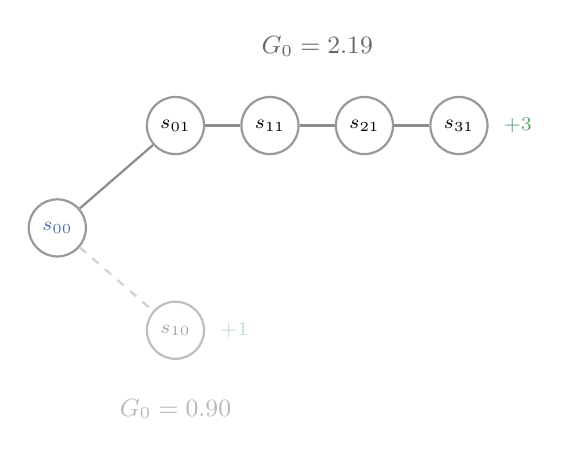
\begin{tikzpicture}
    % Start
    \node[dt node, font=\scriptsize\bfseries, text=agentblue]
        (s0) at (0, 0) {$s_{00}$};
    % Short path (faded)
    \node[dt node, draw=black!25, text=black!35] (r1) at (1.5, -1.3) {$s_{10}$};
    \node[dg reward, text=rewardgreen!40, right=2pt] at (r1.east)
        {$+1$};
    \draw[dt faded] (s0) -- (r1);
    % Long path (taken)
    \node[dt node] (t1) at (1.5, 1.3) {$s_{01}$};
    \node[dt node] (t2) at (2.7, 1.3) {$s_{11}$};
    \node[dt node] (t3) at (3.9, 1.3) {$s_{21}$};
    \node[dt node] (r3) at (5.1, 1.3) {$s_{31}$};
    \node[dg reward, text=rewardgreen, right=2pt] at (r3.east)
        {$+3$};
    \draw[dt taken] (s0) -- (t1);
    \draw[dt taken] (t1) -- (t2);
    \draw[dt taken] (t2) -- (t3);
    \draw[dt taken] (t3) -- (r3);
    % Return annotations
    \node[dt fann, ] at (1.5, -2.3) {$G_0 = 0.90$};
    \node[dt ann] at (3.3, 2.3) {$G_0 = 2.19$};
\end{tikzpicture}
\end{minipage}
\vspace{0.3em}
\subcaption{$\gamma = 0.9$: the distant $+3$ is preferred.}
\label{fig:discount-high}
\end{subfigure}

\vspace{0.5em}
\caption{The discount rate determines which path the agent prefers.
  Left: a grid with a nearby $+1$ and a distant $+3$. Right: the
  same choice as a decision tree with computed returns.}
\label{fig:discounting}
\end{figure}
